\subsection{Rechtwinklige Dreiecke}
\label{subsec:fundamentals_right_triangles}

Rechtwinklige Dreiecke spielen in der Trigonometrie eine zentrale Rolle. An
ihnen werden grundlegende Beziehungen zwischen Seitenlängen und Winkeln
eingeführt.

\begin{DefinitionBox}{Rechtwinkliges Dreieck}{fundamentals_right_triangle}
  Ein \emph{rechtwinkliges Dreieck} \EnglishTerm{right triangle} besitzt einen
  rechten Winkel $\gamma=90^\circ$.
  %
  \begin{center}
    \CachedTikzFigure{content/resources/chapters/fundamentals/tikz/right_triangle_sides.tex}
  \end{center}
  %
  Die dem rechten Winkel gegenüberliegende Seite heißt \emph{Hypotenuse}
  \EnglishTerm{hypotenuse} und ist stets die längste Seite im Dreieck. Die beiden Seiten,
  die den rechten Winkel einschließen, heißen \emph{Katheten} \EnglishTerm{legs}.
\end{DefinitionBox}

\begin{KeyPointBox}{Winkelsumme im rechtwinkligen Dreieck}{fundamentals_right_triangle_angle_sum}
  Wegen $\gamma=90^\circ$ vereinfacht sich die Winkelsumme zu
  \[
      \alpha + \beta + \gamma = 180^\circ
      \qquad\Longrightarrow\qquad
      \Cloze{5cm}{\alpha +\beta =90^\circ}.
  \]
\end{KeyPointBox}

\subsubsection{Satz des Pythagoras}
\label{subsubsec:fundamentals_right_triangles_pythagorean_theorem}

Der Satz des Pythagoras verknüpft die drei Seitenlängen eines rechtwinkligen
Dreiecks. Dabei bezeichnet $c$ die Hypotenuse und $a,b$ die Katheten.

\begin{TheoremBox}{Satz des Pythagoras}{fundamentals_pythagorean_theorem}
  \noindent
  \begin{minipage}[t]{0.64\linewidth}
    Für jedes Dreieck sind die folgenden Aussagen äquivalent:
    \begin{ClozeArea}[22]{3}
      \[
        \begin{gathered}
          \text{Dreieck ist rechtwinklig}\\[-0.1em]
          \gamma=90^\circ
        \end{gathered}
        \quad \Longleftrightarrow \quad
        a^2+b^2=c^2.
      \]
    \end{ClozeArea}
    Dabei ist die Seite $c$ die dem Winkel $\gamma$ gegenüberliegende Seite.
  \end{minipage}\hfill
  \begin{minipage}[t]{0.31\linewidth}
    \vspace{0pt}
    \centering
    \CachedTikzFigure{content/resources/chapters/fundamentals/tikz/right_triangle_pythagorean_example.tex}
  \end{minipage}
\end{TheoremBox}
Aufgrund der Äquivalenz beider Aussagen ist der Satz des Pythagoras nicht nur ein Werkzeug
um Seitenlängen in rechtwinkligen Dreiecken zu berechnen, sondern auch um die
Rechtwinkligkeit eines Dreiecks zu prüfen.

\begin{ExampleBox}{Satz des Pythagoras}{fundamentals_pythagorean_theorem_example}
  \begin{minipage}[c]{0.62\linewidth}
  Gegeben sind die Hypotenuse $c=5\,\mathrm{cm}$ und die Kathete
  $b=4\,\mathrm{cm}$. Gesucht ist die Kathete $a$.
    \begin{ClozeArea}[22]{7}
      \begin{align*}
        \phantom{\Longrightarrow \quad} c^2&=a^2+b^2,\\
        \Longrightarrow \quad a&=\sqrt{c^2-b^2}=\sqrt{(5\,\mathrm{cm})^2-(4\,\mathrm{cm})^2}
         =\sqrt{9\,\mathrm{cm}^2}=3\,\mathrm{cm}.
      \end{align*}
    \end{ClozeArea}
  \end{minipage}\hfill
  \begin{minipage}[c]{0.33\linewidth}
    \centering
    \CachedTikzFigure{content/resources/chapters/fundamentals/tikz/right_triangle_pythagorean_example.tex}
  \end{minipage}
\end{ExampleBox}

\subsubsection{Trigonometrische Funktionen}
\label{subsubsec:fundamentals_right_triangles_trigonometric_ratios}

Bezogen auf einen Winkel $\alpha$ heißen die beiden Katheten Ankathete und
Gegenkathete. Diese Bezeichnungen hängen davon ab, welcher Winkel betrachtet
wird.

\begin{DefinitionBox}{Ankathete und Gegenkathete}{fundamentals_adjacent_and_opposite_leg}
  Die am Winkel $\alpha$ liegende Kathete heißt \emph{Ankathete}
  \EnglishTerm{adjacent leg}. Die dem Winkel $\alpha$ gegenüberliegende
  Kathete heißt \emph{Gegenkathete} \EnglishTerm{opposite leg}.

  \begin{center}
    \CachedTikzFigure{content/resources/chapters/fundamentals/tikz/right_triangle_relative_sides.tex}
  \end{center}
\end{DefinitionBox}

\IfClozeTF{\clearpage}{}
Im rechtwinkligen Dreieck bestimmt das Verhältnis zweier Seiten den
betrachteten spitzen Winkel eindeutig; diesen nichttrivialen Zusammenhang
beschreiben die trigonometrischen Funktionen Sinus, Kosinus und Tangens.

\begin{DefinitionBox}{Sinus, Kosinus und Tangens}{fundamentals_sine_cosine_tangent}
  Die drei grundlegenden trigonometrischen Funktionen sind
  \emph{Sinus} \EnglishTerm{sine}, \emph{Kosinus} \EnglishTerm{cosine} und
  \emph{Tangens} \EnglishTerm{tangent}. Mit ihnen wird aus einem gegebenen
  Winkel das jeweilige Seitenverhältnis berechnet:
  \par\smallskip
  \noindent
  \begin{minipage}[c]{0.54\linewidth}
    \begin{ClozeArea}[18]{8}
      \begin{align*}
        \sin(\alpha)
          &\coloneqq\frac{\text{Gegenkathete}}{\text{Hypotenuse}}
           =\frac{a}{c},\\
        \cos(\alpha)
          &\coloneqq\frac{\text{Ankathete}}{\text{Hypotenuse}}
           =\frac{b}{c},\\
        \tan(\alpha)
          &\coloneqq\frac{\text{Gegenkathete}}{\text{Ankathete}}
           =\frac{a}{b}.
      \end{align*}
    \end{ClozeArea}
  \end{minipage}\hfill
  \begin{minipage}[c]{0.42\linewidth}
    \centering
    \CachedTikzFigure{content/resources/chapters/fundamentals/tikz/right_triangle_relative_sides.tex}
  \end{minipage}
\end{DefinitionBox}

\begin{KeyPointBox}[breakable=false]{Arkusfunktionen}{fundamentals_inverse_trigonometric_ratios}
  Sinus, Kosinus und Tangens berechnen aus einem Winkel ein Seitenverhältnis.
  Die \emph{Arkusfunktionen} kehren diese Zuordnung um: Mit ihnen wird aus
  einem Seitenverhältnis der zugehörige Winkel berechnet.
  \[
    \begin{array}{@{}r@{\qquad}l@{\qquad}c@{\qquad}l@{}}
      \sin(\alpha)=x
      & \TransformOp{\arcsin(\ldots)}
      & \Longleftrightarrow
      & \alpha=\arcsin(x)\\[0.9em]
      \cos(\alpha)=x
      & \TransformOp{\arccos(\ldots)}
      & \Longleftrightarrow
      & \alpha=\arccos(x)\\[0.9em]
      \tan(\alpha)=x
      & \TransformOp{\arctan(\ldots)}
      & \Longleftrightarrow
      & \alpha=\arctan(x)
    \end{array}
  \]
  Auf vielen Taschenrechnern stehen dafür die Tasten
  $\sin^{-1}$, $\cos^{-1}$ und $\tan^{-1}$.
\end{KeyPointBox}

\begin{RemarkBox}[remark title=Winkelmodus des Taschenrechners]
  \noindent
  \begin{minipage}[c]{0.58\linewidth}
    Der Taschenrechner muss wissen, in welchem Winkelmaß eine trigonometrische
    Funktion einen Winkel annimmt bzw. eine Arkusfunktion einen Winkel ausgibt:
    \texttt{DEG} steht für Gradmaß, \texttt{RAD} für Bogenmaß. Mit der Taste
    \texttt{DRG} wechselt man zwischen den Modi. \\
    \begin{equation*}
      \begin{aligned}
      \text{\texttt{DEG}}
        &\;\longleftrightarrow\; \text{Gradmaß }\text{\EnglishTerm{degree measure}},\\
      \text{\texttt{RAD}}
        &\;\longleftrightarrow\; \text{Bogenmaß }\text{\EnglishTerm{radian measure}}.
      \end{aligned}
    \end{equation*}
  \end{minipage}\hfill
  \begin{minipage}[c]{0.38\linewidth}
    \centering
    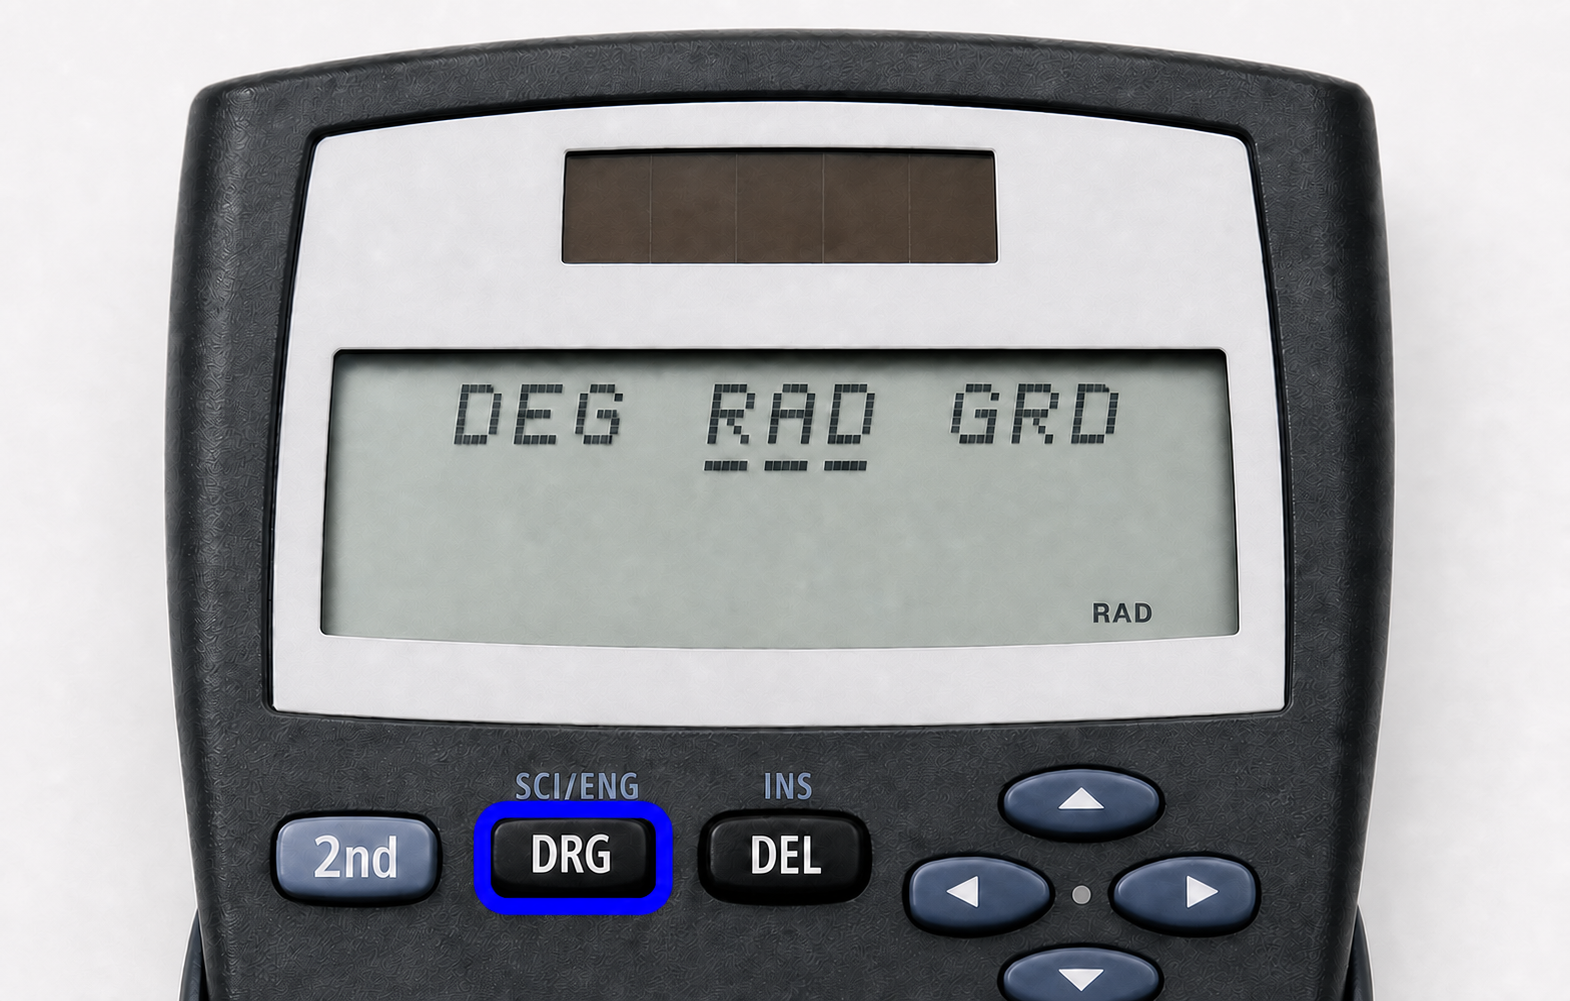
\includegraphics[width=0.82\linewidth]{content/resources/chapters/fundamentals/images/calculator_angle_mode_rad.png}
  \end{minipage}
\end{RemarkBox}

\begin{ExampleBox}{Winkel und Kathete bestimmen}{fundamentals_trigonometric_ratios_example}
  \noindent
  \begin{minipage}[t]{0.72\linewidth}
    \vspace{0pt}
    Gegeben ist ein rechtwinkliges Dreieck mit der Hypotenuse $c=5\,\mathrm{cm}$ und einer Kathete
    $b=4\,\mathrm{cm}$. Gesucht sind der Winkel $\alpha$ und die Kathete $a$. \\

    Wir berechnen zunächst den Winkel $\alpha$. Da $c$, die Hypotenuse, und $b$,
    die Ankathete von $\alpha$, bekannt sind, verwenden wir hierfür die Kosinus-Funktion
    bzw. die Arkus-Kosinus-Funktion:
  \end{minipage}\hfill
  \begin{minipage}[t]{0.24\linewidth}
    \vspace{0pt}
    \centering
    \CachedTikzFigure{content/resources/chapters/fundamentals/tikz/right_triangle_trigonometric_ratios_example.tex}
  \end{minipage}
  %
  \[
    \Cloze{3.1cm}{\cos(\alpha)=\frac{b}{c}}
    \quad\Longrightarrow\quad
    \EquationBranches[\approx]
      {\Cloze{5.8cm}{%
        \alpha=\arccos\!\left(\frac{b}{c}\right)
          =\arccos\!\left(\frac{4\,\mathrm{cm}}{5\,\mathrm{cm}}\right)}}
      {\Cloze{1.6cm}{36{,}9^\circ}}
      {\text{(Gradmaß)}}
      {\Cloze{1.6cm}{0{,}644}}
      {\text{(Bogenmaß)}}
  \]

  Anschließend berechnen wir die Kathete $a$ mit \dots
  \begingroup
  \setlength{\abovedisplayskip}{0.45em}
  \setlength{\abovedisplayshortskip}{0.45em}
  \setlength{\belowdisplayskip}{0.65em}
  \setlength{\belowdisplayshortskip}{0.65em}
  \begin{itemize}[leftmargin=*,topsep=0.35em,itemsep=0pt,parsep=0pt]
    \item der Sinus-Funktion:
      \[
        \Cloze{3.2cm}{\sin(\alpha)=\frac{a}{c}}
        \quad\Longrightarrow\quad
        \Cloze{9.7cm}{%
          a=\sin(\alpha) \cdot c
            =\sin(36{,}9^\circ)\cdot5\,\mathrm{cm}
            \approx3\,\mathrm{cm}}
      \]
    \item der Tangens-Funktion:
      \[
        \Cloze{3.2cm}{\tan(\alpha)=\frac{a}{b}}
        \quad\Longrightarrow\quad
        \Cloze{9.7cm}{%
          a=\tan(\alpha) \cdot b
            =\tan(36{,}9^\circ)\cdot4\,\mathrm{cm}
            \approx3\,\mathrm{cm}}
      \]
    \item dem Satz des Pythagoras:
      \[
        \Cloze{3.2cm}{a^2+b^2=c^2}
        \quad\Longrightarrow\quad
        \Cloze{9.7cm}{%
          a=\sqrt{c^2-b^2}
            =\sqrt{(5\,\mathrm{cm})^2-(4\,\mathrm{cm})^2}
            =3\,\mathrm{cm}}
      \]
  \end{itemize}
  \endgroup
\end{ExampleBox}

\IfClozeTF{}{\clearpage}

\subsubsection{Tangens als Quotient}

Aus den Definitionen der trigonometrischen Funktionen folgt unmittelbar:

\begin{KeyPointBox}{Tangens als Quotient}{fundamentals_tangent_quotient}
  \noindent
  \begin{minipage}[c]{0.73\linewidth}
    Im Quotienten aus Sinus und Kosinus kürzt sich die Hypotenuse $c$ heraus:
    \begin{ClozeArea}[23]{6}
      \[
        \frac{\sin(\alpha)}{\cos(\alpha)}
          =\frac{a/c}{b/c}
           =\frac{a}{b}
           =\tan(\alpha)
        \quad\Longrightarrow\quad
        \tan(\alpha)=\frac{\sin(\alpha)}{\cos(\alpha)}.
      \]
    \end{ClozeArea}
  \end{minipage}\hfill
  \begin{minipage}[c]{0.23\linewidth}
    \centering
    \CachedTikzFigure{content/resources/chapters/fundamentals/tikz/right_triangle_trigonometric_ratios_example.tex}
  \end{minipage}
\end{KeyPointBox}

Damit können wir nun die Werte der Tangensfunktion $\tan(\ldots)$ aus den entsprechenden Sinus- und
Kosinuswerten berechnen.

\IfClozeTF{\clearpage}{}

\subsubsection{Wichtige Winkelwerte}

Für häufig auftretende Winkel sind die Werte der trigonometrischen Funktionen
exakt bekannt:

\begin{center}
  \IfClozeTF
    {\renewcommand{\arraystretch}{2.05}}
    {\renewcommand{\arraystretch}{1.6}}
  \setlength{\tabcolsep}{4pt}
  \begin{tabularx}{\linewidth}{>{\raggedleft\arraybackslash}p{3.6cm}|*{5}{>{\centering\arraybackslash}X}}
    \toprule
    $\alpha$ im Gradmaß
      & $0^\circ$ & $30^\circ$ & $45^\circ$ & $60^\circ$ & $90^\circ$\\
    $\alpha$ im Bogenmaß
      & $0$ & $\frac{\pi}{6}$ & $\frac{\pi}{4}$
      & $\frac{\pi}{3}$ & $\frac{\pi}{2}$\\
    \midrule
    $\sin(\alpha)$
      & \Cloze{2.2cm}{$\frac{\sqrt{0}}{2}\mathrlap{\textcolor{gray}{\, = 0 }}$}
      & \Cloze{2.2cm}{$\frac{\sqrt{1}}{2}\mathrlap{\textcolor{gray}{\, = \frac12 }}$}
      & \Cloze{2.2cm}{$\frac{\sqrt{2}}{2}$}
      & \Cloze{2.2cm}{$\frac{\sqrt{3}}{2}$}
      & \Cloze{2.2cm}{$\frac{\sqrt{4}}{2}\mathrlap{\textcolor{gray}{\, = 1 }}$}\\
    $\cos(\alpha)$
      & \Cloze{2.2cm}{$\frac{\sqrt{4}}{2}\mathrlap{\textcolor{gray}{\, = 1 }}$}
      & \Cloze{2.2cm}{$\frac{\sqrt{3}}{2}$}
      & \Cloze{2.2cm}{$\frac{\sqrt{2}}{2}$}
      & \Cloze{2.2cm}{$\frac{\sqrt{1}}{2}\mathrlap{\textcolor{gray}{\, = \frac12 }}$}
      & \Cloze{2.2cm}{$\frac{\sqrt{0}}{2}\mathrlap{\textcolor{gray}{\, = 0 }}$}\\
    $\tan(\alpha)$
      & \Cloze{1cm}{$0$}
      & \Cloze{1cm}{$\frac{1}{\sqrt3}$}
      & \Cloze{1cm}{$1$}
      & \Cloze{1cm}{$\sqrt3$}
      & \textemdash\\
    \bottomrule
  \end{tabularx}
\end{center}
%

\IfClozeTF{}{\clearpage}

\subsubsection{Trigonometrischer Pythagoras}

Aus dem Satz des Pythagoras folgt eine grundlegende Beziehung zwischen Sinus
und Kosinus.

\begin{KeyPointBox}[breakable=false]{Trigonometrischer Pythagoras}{fundamentals_trigonometric_pythagorean_identity}
  \noindent
  \begin{minipage}[c]{0.68\linewidth}
    Ausgehend vom Satz des Pythagoras gilt:
    \begin{ClozeArea}[21]{8}
      \[
        \begin{array}{@{}c@{\quad}l@{\qquad}l@{}}
          & \vphantom{\left(\frac{a}{c}\right)^2
              +\left(\frac{b}{c}\right)^2}a^2+b^2=c^2
          & \TransformOp{:c^2}\\[0.7em]
          \Longleftrightarrow
          & \vphantom{\left(\frac{a}{c}\right)^2
              +\left(\frac{b}{c}\right)^2}
            \left(\frac{a}{c}\right)^2
            +\left(\frac{b}{c}\right)^2=1
          & \\[0.7em]
          \Longleftrightarrow
          & \vphantom{\left(\frac{a}{c}\right)^2
              +\left(\frac{b}{c}\right)^2}
            \sin^2(\alpha)+\cos^2(\alpha)=1
            \mathrlap{\quad\text{(trigonometrischer Pythagoras)}}
          &
        \end{array}
      \]
    \end{ClozeArea}
  \end{minipage}\hfill
  \begin{minipage}[c]{0.2\linewidth}
    \centering
    \CachedTikzFigure{content/resources/chapters/fundamentals/tikz/right_triangle_pythagorean_example.tex}
  \end{minipage}
\end{KeyPointBox}

\begin{ExampleBox}{Trigonometrischen Pythagoras überprüfen}{fundamentals_trigonometric_pythagorean_identity_example}
  Mit den Werten aus der Tabelle erhalten wir:
  \begin{enumerate}[label=\alph*),leftmargin=2em,labelsep=0.6em,
      topsep=0.4em,itemsep=0.7em]
    \item $\displaystyle
      \sin^2(45^\circ)+\cos^2(45^\circ)
      =\Cloze{9cm}{%
        \left(\frac{\sqrt2}{2}\right)^2
        +\left(\frac{\sqrt2}{2}\right)^2
        =\frac12+\frac12=1
        \quad\mathord{\tikz[x=1ex,y=1ex,baseline=-0.1ex]
          \draw[green!55!black,line width=1.2pt,line cap=round,line join=round]
            (0,0.35)--(0.3,0)--(0.9,0.8);}}$
    \item $\displaystyle
      \sin^2(30^\circ)+\cos^2(30^\circ)
      =\Cloze{9cm}{%
        \left(\frac12\right)^2
        +\left(\frac{\sqrt3}{2}\right)^2
        =\frac14+\frac34=1
        \quad\mathord{\tikz[x=1ex,y=1ex,baseline=-0.1ex]
          \draw[green!55!black,line width=1.2pt,line cap=round,line join=round]
            (0,0.35)--(0.3,0)--(0.9,0.8);}}$
  \end{enumerate}
\end{ExampleBox}


\subsubsection{Additionstheoreme}

Die Additionstheoreme geben Sinus und Kosinus einer Summe oder Differenz zweier
Winkel an.

\begin{TheoremBox}{Additionstheoreme}{fundamentals_trigonometric_addition_formulas}
  \begin{ClozeArea}[34]{8}
    \begin{align*}
      \sin(\alpha\pm\beta)
        &=\sin(\alpha)\cos(\beta)
          \pm\cos(\alpha)\sin(\beta),\\
      \cos(\alpha\pm\beta)
        &=\cos(\alpha)\cos(\beta)
          \mp\sin(\alpha)\sin(\beta).
    \end{align*}
  \end{ClozeArea}
\end{TheoremBox}

Besonders wichig ist der Spezialfall $\beta=\alpha$ für den man Doppelwinkelformeln erhält.

\begin{KeyPointBox}{Doppelwinkelformeln}{fundamentals_trigonometric_double_angle_formulas}
  \begin{ClozeArea}[28]{6}
    \begin{align*}
      \sin(2\alpha)&=2\sin(\alpha)\cos(\alpha),\\
      \cos(2\alpha)&=\cos^2(\alpha)-\sin^2(\alpha).
    \end{align*}
  \end{ClozeArea}
\end{KeyPointBox}


